Леонардо, как и многие другие итальянские ученые и художники его времени, очень интересовался градостроением. Он решил спроектировать идеальный город: комфортабельный, просторный и рациональный в плане использования ресурсов, не такой как тесные и зажатые города средневековья.

Город состоит из $N$ кварталов, расположенных на бесконечной квадратной сетке из клеток. Каждая клетка определяется парой координат (строка, столбец). Для клетки $(i, j)$ соседними являются клетки $(i - 1, j)$, $(i + 1, j)$, $(i, j - 1)$ и $(i, j + 1)$. Каждый квартал занимает на сетке в точности одну клетку. Квартал может занимать клетку $(i, j)$ тогда и только тогда, когда $1 \le i, j \le 2^{31} - 2$. Для обозначения кварталов мы будем использовать координаты соответствующих клеток. Два квартала называются соседними, если они занимают соседние клетки. В идеальном городе все кварталы соединены так, что нет <<дырок>> внутри его границы, то есть, клетки должны удовлетворять следующим условиям:

\begin{itemize}
\item Для любых двух пустых клеток существует не менее одной последовательности соседних между собой пусты клеток, соединяющих эти две клетки.
\item Для любых двух непустых клеток, существует не менее одной последовательности соседних между собой непустых клеток, соединяющих эти две клетки.
\end{itemize}

\bf{Пример 1}

Ни одна из конфигураций кварталов, приведенных ниже, не является идеальным городом: первые две слева не удовлетворяют первому условию, третья не удовлетворяет второму условию, и четвертая не удовлетворяет обоим условиям.

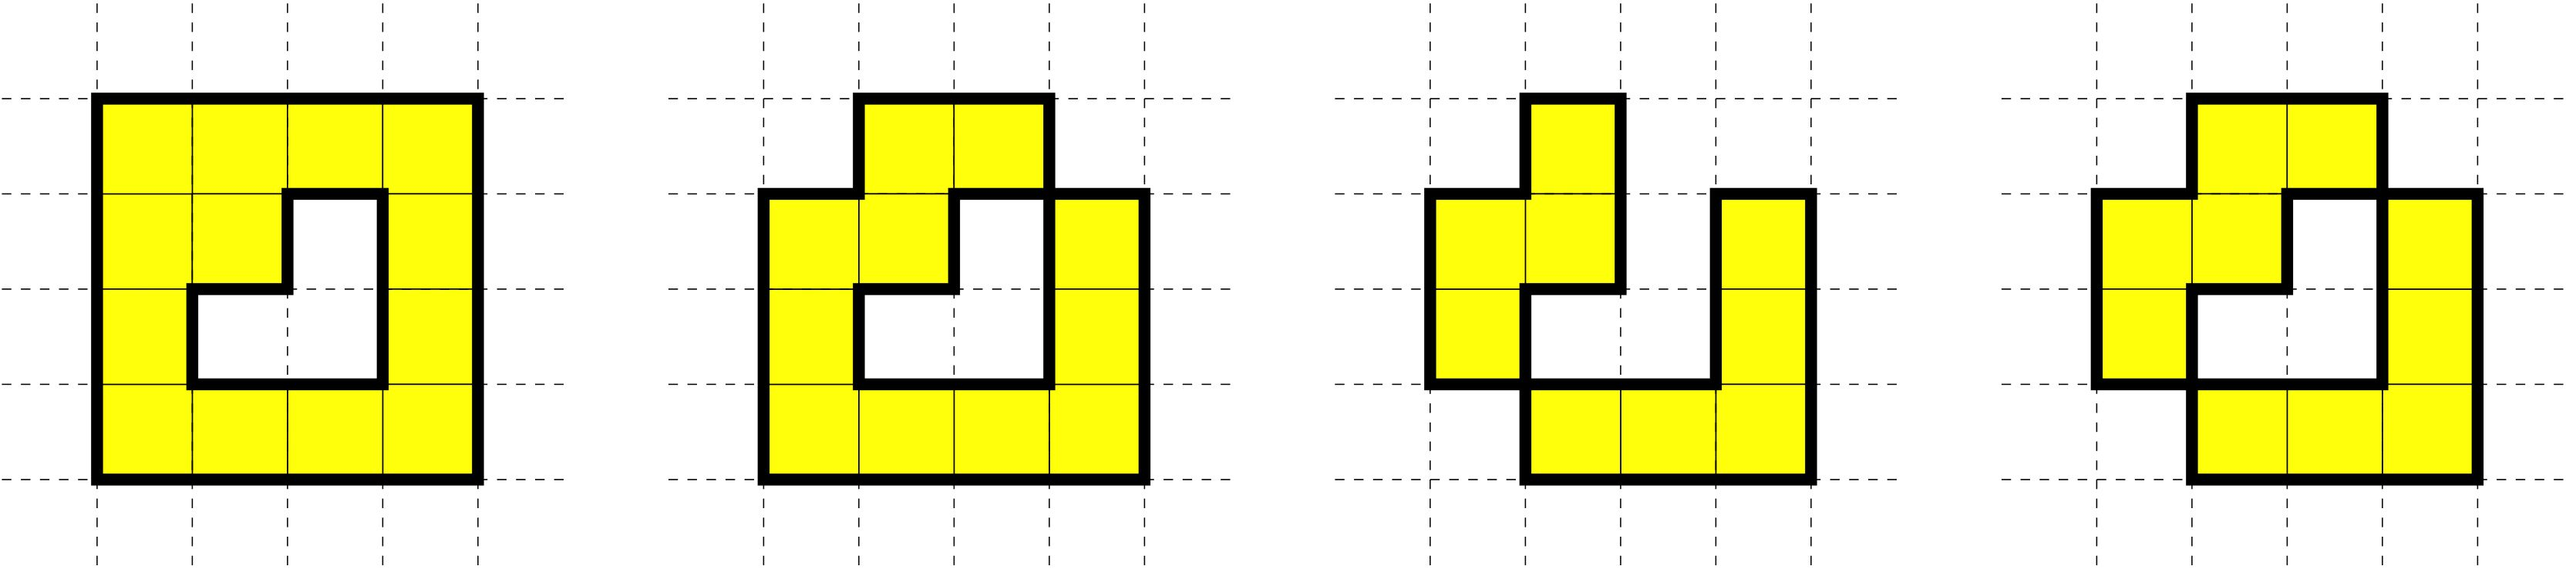
\includegraphics{2012-4-01.jpg}

\bf{Расстояние}

При движении по городу, слово <<прыжок>> обозначает переход от квартала к соседнему. По пустым клеткам нельзя передвигаться. Пусть $v_0, v_1, \dots, v_N$ - это координаты кварталов, расположенных на сетке. Для любых двух различных кварталов с координатами $v_i$ и $v_j$ расстояние $d(v_i, v_j)$ - это минимальное количество прыжков, которое необходимо совершить для перехода от одного квартала к другому.

\bf{Пример 2}

Конфигурация ниже представляет собой идеальный город, состоящий из $N = 11$ кварталов.

\begin{tabular}{crcl}
\multirow{10}{*}{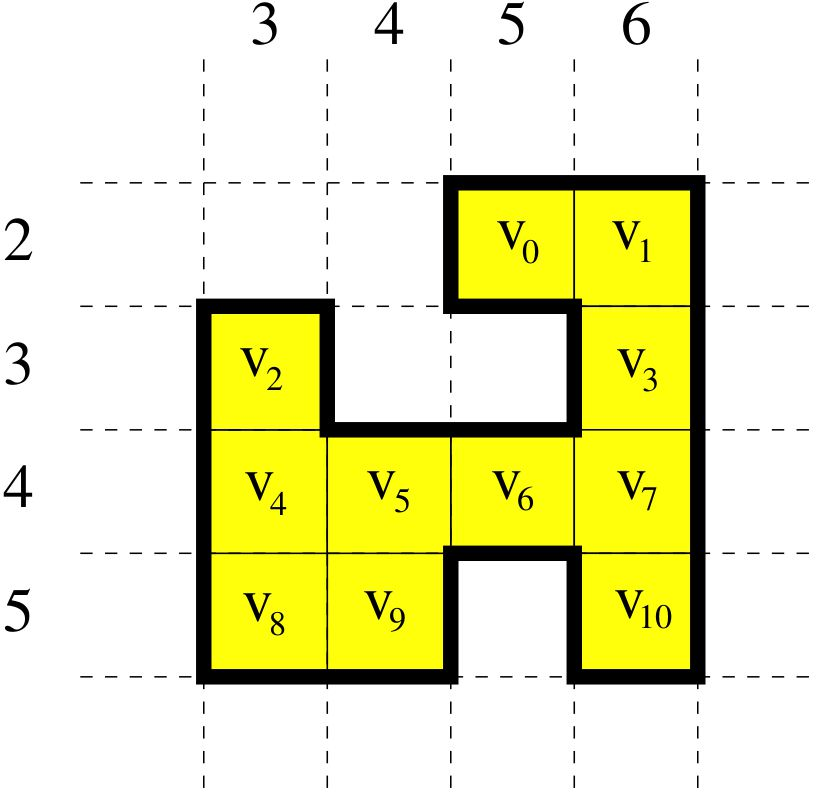
\includegraphics[height = 27ex]{2012-4-02.jpg}}& 
$v_0$ &$=$& $(2,5)$\\
&$v_1$ &$=$& $(2,6)$\\
&$v_2$ &$=$& $(3,3)$\\
&$v_3$ &$=$& $(3,6)$\\
&$v_4$ &$=$& $(4,3)$\\
&$v_5$ &$=$& $(4,4)$\\
&$v_6$ &$=$& $(4,5)$\\
&$v_7$ &$=$& $(4,6)$\\
&$v_8$ &$=$& $(5,3)$\\
&$v_9$ &$=$& $(5,4)$\\
&$v_{10}$ &$=$& $(5,6)$\\
\end{tabular}

Здесь, например, $d(v_1, v_3) = 1$; $d(v_1, v_8) = 6$; и $d(v_9, v_{10}) = 4$.

\bf{Постановка задачи}

Вы должны написать программу, вычисляющую сумму всех попарных расстояний между кварталами идеального города $v_i$ и $v_j$ для каждых $i < j$. То есть, ваша программа должна вычислять значение следующей суммы: 

\begin{center}
$\sum d(v_i, v_j)$; где $0 \le i < j \le N-1$
\end{center}

А именно, вы должны реализовать процедуру \t{DistanceSum(N, X, Y)} которая, по заданным $N$ и двум массивам $X$ и $Y$, которые описывают город, вычисляет значение по формуле выше. Массивы как $X$ так и $Y$ содержат $N$ элементов; Квартал $i$ имеет координаты $(X[i], Y[i])$ для $0 \le i \le N - 1$ и $1 \le X[i], Y[i] \le 2^{31} - 2$. Поскольку результат может быть слишком большим, чтобы вместиться в 32 бита, вы должны вывести это число по модулю $1\,000\,000\,000$ (один миллиард). В примере 2, имеется $\frac{11 × 10}{2} = 55$ пар кварталов. Сумма всех попарных расстояний равна $174$.

\bf{Детали реализации}

Вы должны отправить на проверку один файл с названием \t{city.c}, \t{city.cpp} или \t{city.pas}. Этот файл должен реализовывать процедуру, описанную выше, используя следующее описание (сигнатуру):

\begin{itemize}
\item Реализация на C/C++:

\t{int DistanceSum(int N, int *X, int *Y);}
\item Реализация на Pascal:

\t{function DistanceSum(N : LongInt; var X, Y : array of LongInt) : LongInt;}
\end{itemize}

Эти процедуры должны вести себя как описано выше. Конечно, вы можете реализовывать любые другие процедуры для внутреннего использования. Отправляемое вами решение не должно никаким образом взаимодействовать со стандартным потоком ввода/вывода или любым другим файлом.

\bf{Пример проверяющего модуля (grader)}

Предоставляемый пример проверяющего модуля (grader) использует следующий формат ввода:
\begin{itemize}
\item строка 1: $N$;
\item строки 2, \ldots, N + 1: $X[i]$, $Y[i]$.
\end{itemize}
